
\section*{Average Temperature.}
The average temperature is calculated by taking in the sum of the temperature each day and then dividing by the number of days considerer which is done with a simple for loop.

\begin{figure}
	\centering
	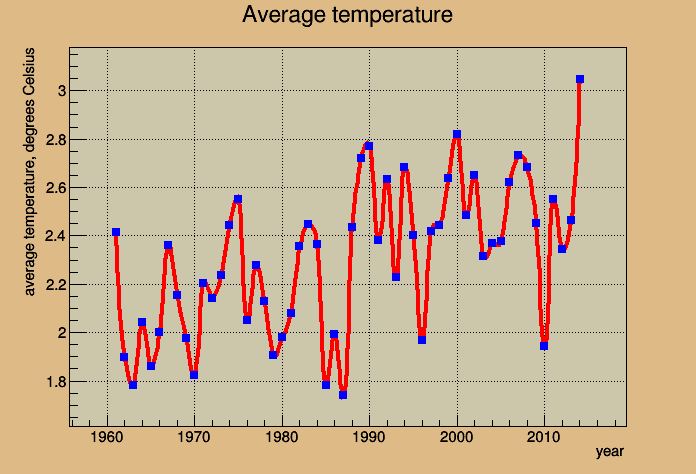
\includegraphics[width=0.8 \textwidth]{lund.png}
	\caption{Average temperature for each year measured in Lund.}
\end{figure}
In figure 1 one can see the the average temperature for every year for each weather station. 
The function works by taking the two dimensional array of the temperature per day per year, the number of years considered, the threshold for discarding elements and the array where the average temperatures are going to be stored. It runs them through a \texttt{for} loop checking whether the temperature for a certain day is reliable, if its not it will be taken into account  when calculating the average temperature. It will discard the unreliable values by a \texttt{if} statement that states if the element is smaller than the threshold it will be discarded(this is a feature of the reading).